\documentclass[12pt]{article}
\usepackage{takeaway}
\setband{Kindergarten \& Grade 1}

% ---- K-1 helpers ----
\newcommand{\crown}[2]{% \crown{(x,y)}{size}
  \begin{scope}[shift={#1},scale=#2]
  \fill[orange] (-0.5,0) -- (-0.55,0.55) -- (-0.25,0.25) -- (0,0.65) -- (0.25,0.25) -- (0.55,0.55) -- (0.5,0) -- cycle;
  \fill[white] (0,0.12) circle (0.07);
  \end{scope}}
\newcommand{\checkmk}[2]{% \checkmk{(x,y)}{size}
  \draw[teal,line width=2.4pt,line cap=round,line join=round,shift={#1},scale=#2]
    (-0.3,0.02) -- (-0.08,-0.22) -- (0.32,0.3);}
\newcommand{\xmk}[2]{%
  \draw[orange,line width=2.4pt,line cap=round,shift={#1},scale=#2]
    (-0.28,-0.28) -- (0.28,0.28) (-0.28,0.28) -- (0.28,-0.28);}
% the "circle one" pair: \choice{(x,y)}
\newcommand{\choice}[1]{%
  \begin{scope}[shift={#1}]
  \smiley{(0,0.1)}{0.55}
  \node[font=\fontsize{12}{13}\selectfont\subheadfont,text=teal] at (0,-0.75) {I can win};
  \trapweb{(2.2,0.1)}{0.55}
  \node[font=\fontsize{12}{13}\selectfont\subheadfont,text=orange] at (2.2,-0.75) {trap};
  \end{scope}}
\newcommand{\bignum}[2]{% \bignum{(x,y)}{n}
  \node[circle,draw=teal,line width=1.4pt,fill=white,minimum size=1.25cm,font=\headfont\fontsize{24}{24}\selectfont,text=teal] at #1 {#2};}

\begin{document}
\fontsize{17}{22}\selectfont

%=====================================================================
\bigtitle{Take the Last One!}{A counter game for two players}
\nameline[My name]

\vspace{4pt}
\begin{center}
\begin{tikzpicture}[x=1cm,y=1cm]
  % three picture panels
  \foreach \p/\t in {0/{Make a pile.},6.1/{Take turns.\\Take 1 or 2.},12.2/{Take the last one.\\You win!}}{%
    \draw[orange,line width=1.2pt,fill=orangesoft,rounded corners=4mm] (\p,0) rectangle ++(5.8,4.6);
    \node[align=center,font=\fontsize{16}{19}\selectfont\subheadfont,text=ink] at (\p+2.9,0.75) {\t};
  }
  \node[circle,fill=orange,text=white,font=\subheadfont,minimum size=0.75cm] at (0.45,4.15) {1};
  \node[circle,fill=orange,text=white,font=\subheadfont,minimum size=0.75cm] at (6.55,4.15) {2};
  \node[circle,fill=orange,text=white,font=\subheadfont,minimum size=0.75cm] at (12.65,4.15) {3};
  % panel 1: a pile
  \foreach \x/\y in {2.0/2.0,2.65/2.0,3.3/2.0,3.95/2.0,2.33/2.55,2.98/2.55,3.63/2.55,2.65/3.1,3.3/3.1}{\ctr{(\x,\y)}{0.3}}
  % panel 2: 1 ok, 2 ok, 3 not ok
  \ctr{(7.3,2.6)}{0.26}
  \checkmk{(7.3,3.45)}{0.8}
  \ctr{(8.55,2.6)}{0.26}\ctr{(9.15,2.6)}{0.26}
  \checkmk{(8.85,3.45)}{0.8}
  \ctr{(10.15,2.6)}{0.26}\ctr{(10.7,2.6)}{0.26}\ctr{(11.25,2.6)}{0.26}
  \draw[orange,line width=2.4pt,line cap=round] (9.75,2.25) -- (11.65,2.95) (9.75,2.95) -- (11.65,2.25);
  \node[font=\fontsize{11}{12}\selectfont\subheadfont,text=orange] at (10.7,3.45) {no!};
  \node[font=\subheadfont\fontsize{13}{14}\selectfont,text=teal] at (7.3,2.0) {1};
  \node[font=\subheadfont\fontsize{13}{14}\selectfont,text=teal] at (8.85,2.0) {2};
  \node[font=\subheadfont\fontsize{13}{14}\selectfont,text=orange] at (10.7,2.0) {3};
  % panel 3: last counter with a crown
  \ctr{(15.1,2.3)}{0.42}
  \crown{(15.1,2.85)}{0.95}
\end{tikzpicture}
\end{center}

\vspace{2pt}
{\subheadfont Play here!} Put counters in the circles. Take them off from the end.\\
Start with 5 counters. Then try 7. Then try 10.

\begin{center}
\begin{tikzpicture}[x=1cm,y=1cm]
  % ten frame sized for real counters (spots 2.8 cm across)
  \draw[teal,line width=1.6pt,fill=tealsoft,rounded corners=2mm] (-0.2,-0.2) rectangle (15.7,6.4);
  \foreach \r in {0,1}{\foreach \c in {0,...,4}{%
    \draw[teal!60,line width=0.8pt,fill=white] (\c*3.1+0.05,\r*3.1+0.05) rectangle ++(3.0,3.0);
    \draw[faint,line width=0.8pt,dashed] (\c*3.1+1.55,\r*3.1+1.55) circle (1.25);
  }}
\end{tikzpicture}
\end{center}

\vspace{2pt}
{\subheadfont Who took the last one?} Make a mark for each win.

\begin{center}

\begin{tikzpicture}[x=1cm,y=1cm]
  \draw[teal,line width=1.2pt,rounded corners=3mm] (0,0) rectangle (8.4,2.6);
  \node[font=\subheadfont\fontsize{16}{18}\selectfont,text=teal,anchor=west] at (0.3,2.1) {Me};
  \draw[orange,line width=1.2pt,rounded corners=3mm] (9.4,0) rectangle (17.8,2.6);
  \node[font=\subheadfont\fontsize{16}{18}\selectfont,text=orange,anchor=west] at (9.7,2.1) {My friend};
\end{tikzpicture}
\end{center}

{\fontsize{13}{16}\selectfont\color{grid} Three friends? Two play and one is the helper. Switch after each game.\par}

\newpage
%=====================================================================
\pagetitle{Tiny piles}
It is {\subheadfont YOUR} turn. Can you win? Use real counters to find out!\\[3pt]
Circle the smile \tikz[baseline=-0.6ex]{\smiley{(0,0)}{0.28}} if you can win.\\[3pt]
Circle the web \tikz[baseline=-0.6ex]{\trapweb{(0,0)}{0.28}} if you can't win.

\vspace{6pt}
\begin{center}
\begin{tikzpicture}[x=1cm,y=1cm]
  % pile of 1
  \draw[teal,line width=1.2pt,rounded corners=4mm,fill=tealsoft] (0,0) rectangle (18,2.8);
  \bignum{(1.0,1.4)}{1}
  \ctrrow{1}{2.9}{1.4}{0.5}{1.2}
  \choice{(13.6,1.5)}
  % pile of 2
  \begin{scope}[yshift=-3.25cm]
  \draw[teal,line width=1.2pt,rounded corners=4mm,fill=tealsoft] (0,0) rectangle (18,2.8);
  \bignum{(1.0,1.4)}{2}
  \ctrrow{2}{2.9}{1.4}{0.5}{1.2}
  \choice{(13.6,1.5)}
  \end{scope}
  % pile of 3
  \begin{scope}[yshift=-11.0cm]
  \draw[teal,line width=1.2pt,rounded corners=4mm,fill=tealsoft] (0,0) rectangle (18,7.3);
  \bignum{(1.0,5.9)}{3}
  \ctrrow{3}{2.9}{5.9}{0.5}{1.2}
  \choice{(13.6,6.0)}
  \node[anchor=west,font=\subheadfont\fontsize{16}{18}\selectfont] at (0.5,4.45) {Try it! Draw what your friend gets.};
  % try boxes
  \foreach \bx/\k in {0.5/1,9.3/2}{%
    \draw[orange,line width=1pt,fill=white,rounded corners=3mm] (\bx,0.4) rectangle ++(8.2,3.4);
    \node[anchor=west,font=\fontsize{15}{17}\selectfont] at (\bx+0.3,3.25) {I take \k.};
    \node[anchor=west,font=\fontsize{15}{17}\selectfont] at (\bx+0.3,2.55) {My friend};
    \node[anchor=west,font=\fontsize{15}{17}\selectfont] at (\bx+0.3,1.95) {gets:};
    \draw[faint,line width=0.8pt,dashed,rounded corners=2mm] (\bx+3.3,0.7) rectangle (\bx+7.9,3.5);
  }
  \end{scope}
\end{tikzpicture}
\end{center}

\vspace{6pt}
\begin{ideabox}[Traps]
A {\subheadfont TRAP} is a pile you do not want on your turn.\\[2pt]
Which tiny pile is a trap?
\tikz[baseline=0.4cm]{\draw[orange,line width=1.4pt,rounded corners=2mm,fill=white] (0,0) rectangle (1.6,1.2); \trapweb{(2.3,0.6)}{0.45}}
\end{ideabox}

\newpage
%=====================================================================
\pagetitle{Trap hunt}
\begin{ideabox}[Remember]
\tikz[baseline=-0.6ex]{\trapweb{(0,0)}{0.3}}\ \ 3 is a trap. Give your friend a trap and you can win!\\[2pt]
Can you take 1 or 2 and leave a trap? Write how many you take.\\[2pt]
No way to leave a trap? Then this pile is a trap too!
\end{ideabox}

\vspace{2pt}
\begin{center}
\begin{tikzpicture}[x=1cm,y=1cm]
  \node[font=\subheadfont\fontsize{13}{14}\selectfont,text=grid] at (10.6,0.55) {I take};
  \node[font=\subheadfont\fontsize{13}{14}\selectfont,text=grid] at (15.2,0.55) {circle one};
  \foreach \n [count=\i from 0] in {4,5,6,7,8,9}{%
    \begin{scope}[yshift=-\i*2.45cm]
    \draw[teal!50,line width=0.8pt,rounded corners=3mm] (0,-2.25) rectangle (18,0.05);
    \bignum{(0.95,-1.1)}{\n}
    \ctrrow{\n}{2.45}{-1.1}{0.33}{0.8}
    \draw[ink,line width=1pt,fill=white,rounded corners=1.5mm] (9.95,-1.75) rectangle ++(1.3,1.3);
    \choice{(14.1,-1.0)}
    \end{scope}}
  % worked example in the first row (pile of 4)
  \node[font=\headfont\fontsize{22}{22}\selectfont,text=plum] at (10.6,-1.1) {1};
  \draw[plum,line width=1.4pt] (14.1,-1.2) ellipse (1.25 and 1.0);
  \node[font=\fontsize{11}{12}\selectfont\itshape,text=plum,align=center] at (11.95,-1.1) {friend\\gets 3};
\end{tikzpicture}
\end{center}

\vspace{2pt}
{\subheadfont Circle the traps you found. What comes next?}

\begin{center}
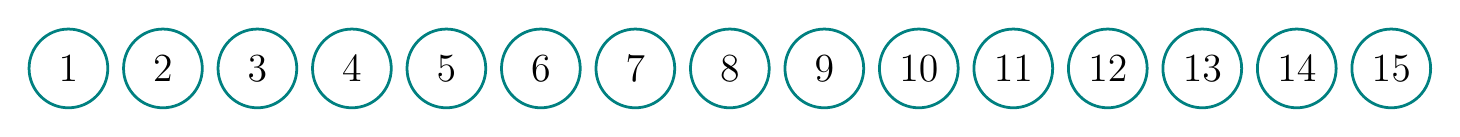
\begin{tikzpicture}[x=1cm,y=1cm]
  \foreach \n in {1,...,15}{%
    \node[circle,draw=teal,line width=1pt,inner sep=0pt,minimum size=1.0cm,font=\subheadfont\fontsize{15}{15}\selectfont] at (\n*1.2-1.2,0) {\n};}
\end{tikzpicture}
\end{center}

\newpage
%=====================================================================
\pagetitle{Trap your grown-up!}
Play against your grown-up. Before each game, {\subheadfont you choose}:\\
go {\subheadfont first} or go {\subheadfont second}?
Try to give the grown-up a trap every time.

\vspace{4pt}
\begin{center}
\begin{tikzpicture}[x=1cm,y=1cm]
  \node[font=\subheadfont\fontsize{13}{14}\selectfont,text=grid] at (2.9,0.5) {start with};
  \node[font=\subheadfont\fontsize{13}{14}\selectfont,text=grid] at (11.1,0.5) {I went (circle)};
  \node[font=\subheadfont\fontsize{13}{14}\selectfont,text=grid] at (15.9,0.5) {I won? (circle)};
  \foreach \n [count=\i from 0] in {5,6,8,9}{%
    \begin{scope}[yshift=-\i*2.35cm]
    \draw[teal!50,line width=0.8pt,rounded corners=3mm] (0,-2.15) rectangle (18,0.05);
    \bignum{(0.95,-1.05)}{\n}
    \ctrrow{\n}{2.4}{-1.05}{0.3}{0.72}
    \node[draw=ink,line width=0.8pt,rounded corners=2mm,font=\subheadfont\fontsize{15}{16}\selectfont,minimum width=1.9cm,minimum height=0.9cm] at (10.1,-1.05) {first};
    \node[draw=ink,line width=0.8pt,rounded corners=2mm,font=\subheadfont\fontsize{15}{16}\selectfont,minimum width=1.9cm,minimum height=0.9cm] at (12.3,-1.05) {second};
    \smiley{(15.2,-1.05)}{0.5}
    \node[font=\fontsize{13}{14}\selectfont,text=grid] at (16.8,-1.05) {not yet};
    \end{scope}}
  % a row where the child picks the start
  \begin{scope}[yshift=-4*2.35cm]
  \draw[plum!60,line width=0.8pt,rounded corners=3mm] (0,-2.15) rectangle (18,0.05);
  \draw[plum,line width=1.4pt,fill=white] (0.95,-1.05) circle (0.62);
  \node[font=\fontsize{15}{17}\selectfont\subheadfont,text=plum,anchor=west] at (2.3,-1.05) {You pick the start!};
  \node[draw=ink,line width=0.8pt,rounded corners=2mm,font=\subheadfont\fontsize{15}{16}\selectfont,minimum width=1.9cm,minimum height=0.9cm] at (10.1,-1.05) {first};
  \node[draw=ink,line width=0.8pt,rounded corners=2mm,font=\subheadfont\fontsize{15}{16}\selectfont,minimum width=1.9cm,minimum height=0.9cm] at (12.3,-1.05) {second};
  \smiley{(15.2,-1.05)}{0.5}
  \node[font=\fontsize{13}{14}\selectfont,text=grid] at (16.8,-1.05) {not yet};
  \end{scope}
\end{tikzpicture}
\end{center}

\vspace{6pt}
\begin{challengebox}[New rule!]

\begin{tikzpicture}[x=1cm,y=1cm,baseline=0]
  \node[anchor=west,font=\subheadfont\fontsize{17}{20}\selectfont] at (0,0.1) {Now you may take 1, 2, or 3.};
  \ctr{(9.3,0.1)}{0.26}
  \ctr{(10.6,0.1)}{0.26}\ctr{(11.2,0.1)}{0.26}
  \ctr{(12.5,0.1)}{0.26}\ctr{(13.1,0.1)}{0.26}\ctr{(13.7,0.1)}{0.26}
  \checkmk{(9.3,0.85)}{0.6}\checkmk{(10.9,0.85)}{0.6}\checkmk{(13.1,0.85)}{0.6}
\end{tikzpicture}

\vspace{6pt}
Play it. Is 3 still a trap?\quad
\tikz[baseline=-0.5ex]{\node[draw=ink,rounded corners=2mm,minimum width=1.5cm,font=\subheadfont] {yes};}\quad
\tikz[baseline=-0.5ex]{\node[draw=ink,rounded corners=2mm,minimum width=1.5cm,font=\subheadfont] {no};}

\vspace{6pt}
Find the new traps. Circle them.

\vspace{4pt}
\centering
\begin{tikzpicture}[x=1cm,y=1cm]
  \foreach \n in {1,...,12}{%
    \node[circle,draw=plum,line width=1pt,fill=white,inner sep=0pt,minimum size=1.0cm,font=\subheadfont\fontsize{15}{15}\selectfont] at (\n*1.3-1.3,0) {\n};}
\end{tikzpicture}
\end{challengebox}

\end{document}
